\documentclass[11pt,a4paper]{article}

\usepackage[utf8]{inputenc}
\usepackage[T1]{fontenc}
\usepackage{lmodern}
\usepackage[margin=1in]{geometry}
\usepackage{titlesec}
\usepackage{xcolor}
\usepackage{parskip}
\usepackage{hyperref}
\usepackage{float} % for table and image placement
\usepackage{graphicx} % for images
\usepackage{titlesec} % for extra subsections
\usepackage{listings} % for code

\definecolor{primary}{RGB}{33, 33, 33}
\definecolor{secondary}{RGB}{85, 85, 85}

\newcommand{\postapi}{\textcolor{green}{POST}}
\newcommand{\getapi}{\textcolor{blue}{GET}}
\newcommand{\putapi}{\textcolor{orange}{PUT}}
\newcommand{\deleteapi}{\textcolor{red}{DELETE}}

\newcommand{\matchmaking}[1]{/api/v1/matchmaking#1}
\newcommand{\ranking}[1]{/api/v1/ranking#1}
\newcommand{\history}[1]{/api/v1/history#1}
\newcommand{\riot}[1]{/api/v1/riot#1}
\newcommand{\training}[1]{/api/v1/training#1}
\newcommand{\analysis}[1]{/api/v1/analysis#1}

\newcommand{\bff}[1]{\textbf{#1}}

\setcounter{secnumdepth}{4}

\titleformat{\section}
{\normalfont\Large\bfseries\color{primary}}{\thesection}{1em}{}
\titleformat{\subsection}
{\normalfont\large\bfseries\color{secondary}}{\thesubsection}{1em}{}
\titleformat{\subsubsection}
{\normalfont\normalsize\bfseries\color{secondary}}{\thesubsubsection}{1em}{}
\titleformat{\paragraph}
{\normalfont\normalsize\bfseries\color{secondary}}{\theparagraph}{1em}{}
\titlespacing*{\paragraph}
{0pt}{3.25ex plus 1ex minus .2ex}{1.5ex plus .2ex}

\setlength{\parskip}{0.8em}
\setlength{\parindent}{0pt}

\title{\vspace{-2cm}\textbf{\Huge Final Report}\vspace{0.5cm}}
\author{
    \textbf{Group 21} \\
    Diogo Sousa fc59792 \\
    Bruno Faustino fc59784 \\
    Rodrigo Neto fc59850
}
\date{\today}

\begin{document}

    \maketitle
    \thispagestyle{empty}
    \tableofcontents
    \listoffigures
    \listoftables

    \vspace{1cm}
    \hrule
    \vspace{1cm}

    %%%%%%%%%%%%%%%%%%%%%%%%%%%%%% Motivation %%%%%%%%%%%%%%%%%%%%%%%%%%%%%%%%%
    \section{Motivation}

    TODO

    \vspace{1cm}
    \hrule
    \vspace{1cm}

    %%%%%%%%%%%%%%%%%%%%%%%%% Dataset Characterization %%%%%%%%%%%%%%%%%%%%%%%%
    \section{Dataset Characterization}

    \begin{itemize}
        \item \bff{Topic}: League of Legends Matches
        \item \bff{URL}: \href{https://www.kaggle.com/datasets/omaracornejo/matches-raw-euw?select=opgg_table_scraper.py}{Kaggle - Matches Raw EUW}
        \item \bff{Size}: Approximately 78 GB
        \item \bff{Release Date}: January 2026
    \end{itemize}

    \vspace{1cm}
    \hrule
    \vspace{1cm}

    %%%%%%%%%%%%%%%%%%%%%%%%% Business Capabilities %%%%%%%%%%%%%%%%%%%%%%%%%%%
    \section{Business Capabilities}

    \subsection{Competitive Ranking}
    
    Facilitates real-time visualization of global and local leaderboards. Includes simplified performance metrics such as Damage dealt and KDA ratios.
    
    \subsection{Custom Match Management}
    
    Enables the creation of balanced custom matches. Matchmaking is handled via a global/local queue system integrated with the project's ranking logic.
    
    \subsection{Custom Match History}
    
    Provides a centralized repository for past custom match statistics. Includes robust functionality for custom filtering and sorting based on specific user requirements.
    
    \subsection{Team Draft and Build Analyzer}
    
    Offers personalized post-game analysis. Players utilizing the API receive automated insights regarding gameplay performance and actionable tips for improvement.

    \vspace{1cm}
    \hrule
    \vspace{1cm}

    %%%%%%%%%%%%%%%%%%%%%%%%%%%%%% Use Cases %%%%%%%%%%%%%%%%%%%%%%%%%%%%%%%%%%
    \section{Use Cases}

    \subsection{Match \& Ranking Management}

    \begin{table}[H]
    \begin{tabular}{|p{10cm}|p{5cm}|}
    \hline
    \bff{Use Case}        & \bff{Student Name} \\ \hline                                      
    Leaderboards          & Diogo Sousa \\ \hline
    User Ranking          & Diogo Sousa \\ \hline
    Match Finding         & Diogo Sousa \\ \hline
    Create / Cancel Match & Diogo Sousa \\ \hline
    \end{tabular}
    \caption{Match \& Ranking Management Use Cases per Student}
    \label{tab:use-cases-match-ranking-management}
    \end{table}

    \subsection{Data Visualization \& Analysis}

    \begin{table}[H]
    \begin{tabular}{|p{10cm}|p{5cm}|}
    \hline
    \bff{Use Case}                                            & \bff{Student Name} \\ \hline                                       
    Match History                                             & Bruno Faustino \\ \hline
    Advanced History Filtering / Sorting / Paging             & Bruno Faustino \\ \hline
    Automatic Detail Filling (by interacting with RIOT's API) & Bruno Faustino \\ \hline
    Draft Analysis                                            & Rodrigo Neto \\ \hline
    Build Analysis                                            & Rodrigo Neto \\ \hline
    Player Performance Analysis                               & Rodrigo Neto \\ \hline
    \end{tabular}
    \caption{Data Visualization \& Analysis Use Cases per Student}
    \label{tab:use-cases-data-visualization-analysis}
    \end{table}

    \vspace{1cm}
    \hrule
    \vspace{1cm}

    %%%%%%%%%%%%%%%%%%%%%%%%%%% API Specification %%%%%%%%%%%%%%%%%%%%%%%%%%%%%
    \section{API Specification}


    \subsection{Player Management - Diogo Sousa}

    Brief Description

    \begin{table}[H]
    \begin{tabular}{|p{2cm}|p{5cm}|p{7cm}|}
    \hline
    \bff{Verb} & \bff{Endpoint}                                          & \bff{Description} \\ \hline
    \postapi   & \url{\matchmaking{/players}}                            & TODO \\ \hline
    \getapi    & \url{\matchmaking{/players/{id}}}                       & TODO \\ \hline
    \getapi    & \url{\matchmaking{/players/{id}/lobbies}}               & TODO \\ \hline
    \getapi    & \url{\matchmaking{/players/{id}/tickets}}               & TODO \\ \hline
    \deleteapi & \url{\ranking{/players/links/{gameName}/{tagLine}}}     & TODO \\ \hline
    \getapi    & \url{\ranking{/players/{playerId}}}                     & TODO \\ \hline
    \putapi    & \url{\ranking{/players/{playerId}/link-lol-account}}    & TODO \\ \hline
    \getapi    & \url{\ranking{/players/{playerId}/primary-account}}     & TODO \\ \hline
    \putapi    & \url{\ranking{/players/{playerId}/set-primary-account}} & TODO \\ \hline
    \postapi   & \url{\ranking{/players/{playerId}/sync-mmr}}            & TODO \\ \hline
    \end{tabular}
    \caption{Player Management REST API}
    \label{tab:api-player-management}
    \end{table}

    \subsection{Queue Management - Diogo Sousa}

    Brief Description

    \begin{table}[H]
    \begin{tabular}{|p{2cm}|p{5cm}|p{7cm}|}
    \hline
    \bff{Verb} & \bff{Endpoint}                   & \bff{Description} \\ \hline
    \postapi   & \url{\matchmaking{/queues}}      & TODO \\ \hline
    \getapi    & \url{\matchmaking{/queues/{id}}} & TODO \\ \hline
    \putapi    & \url{\ranking{/queue/{queueId}}} & TODO \\ \hline
    \getapi    & \url{\ranking{/queue/{queueId}}} & TODO \\ \hline
    \deleteapi & \url{\ranking{/queue/{queueId}}} & TODO \\ \hline
    \end{tabular}
    \caption{Queue Management REST API}
    \label{tab:api-queue-management}
    \end{table}

    \subsection{Matchmaking - Diogo Sousa}

    Brief Description

    \begin{table}[H]
    \begin{tabular}{|p{2cm}|p{5cm}|p{7cm}|}
    \hline
    \bff{Verb} & \bff{Endpoint}                                                            & \bff{Description} \\ \hline
    \postapi   & \url{\matchmaking{/tickets}}                                              & TODO \\ \hline
    \postapi   & \url{\matchmaking{/tickets/matches/{matchId}/complete}}                   & TODO \\ \hline
    \putapi    & \url{\matchmaking{/tickets/matches/{matchId}/link}}                       & TODO \\ \hline
    \postapi   & \url{\matchmaking{/tickets/matches/{matchId}/players/{playerId}/accept}}  & TODO \\ \hline
    \postapi   & \url{\matchmaking{/tickets/matches/{matchId}/players/{playerId}/decline}} & TODO \\ \hline
    \deleteapi & \url{\matchmaking{/tickets/{ticketId}}}                                   & TODO \\ \hline
    \getapi    & \url{\matchmaking{/tickets/{ticketId}/lobby}}                             & TODO \\ \hline
    \end{tabular}
    \caption{Matchmaking REST API}
    \label{tab:api-matchmaking}
    \end{table}

    \subsection{Leaderboard - Diogo Sousa}

    Brief Description

    \begin{table}[H]
    \begin{tabular}{|p{2cm}|p{5cm}|p{7cm}|}
    \hline
    \bff{Verb} & \bff{Endpoint}                                 & \bff{Description} \\ \hline
    \getapi    & \url{\ranking{/leaderboards}}                  & TODO \\ \hline
    \getapi    & \url{\ranking{/leaderboards/queues/{queueId}}} & TODO \\ \hline
    \end{tabular}
    \caption{Leaderboard REST API}
    \label{tab:api-leaderboard}
    \end{table}

    \subsection{Player Ranking - Diogo Sousa}

    Brief Description

    \begin{table}[H]
    \begin{tabular}{|p{2cm}|p{5cm}|p{7cm}|}
    \hline
    \bff{Verb} & \bff{Endpoint}                                              & \bff{Description} \\ \hline
    \getapi    & \url{\ranking{/players/{playerId}/queue-rankings}}          & TODO \\ \hline
    \getapi    & \url{\ranking{/players/{playerId}/queue-rankings{queueId}}} & TODO \\ \hline
    \end{tabular}
    \caption{Player Ranking REST API}
    \label{tab:api-player-ranking}
    \end{table}

    \subsection{Match History - Bruno Faustino}

    Brief Description

    \begin{table}[H]
    \begin{tabular}{|p{2cm}|p{5cm}|p{7cm}|}
    \hline
    \bff{Verb} & \bff{Endpoint}                         & \bff{Description} \\ \hline
    \getapi    & \url{\history{/matches}}               & TODO \\ \hline
    \getapi    & \url{\history{/matches/{riotMatchId}}} & TODO \\ \hline
    \end{tabular}
    \caption{Match History REST API}
    \label{tab:api-match-history}
    \end{table}

    \subsection{Match Filling - Bruno Faustino}

    Brief Description

    \begin{table}[H]
    \begin{tabular}{|p{2cm}|p{5cm}|p{7cm}|}
    \hline
    \bff{Verb} & \bff{Endpoint}                      & \bff{Description} \\ \hline
    \getapi    & \url{\riot{/matches/{matchId}}}     & TODO \\ \hline
    \getapi    & \url{\riot{/matches/{matchId}/raw}} & TODO \\ \hline
    \end{tabular}
    \caption{Match Filling REST API}
    \label{tab:api-match-filling}
    \end{table}

    \subsection{Player Filling - Bruno Faustino}

    Brief Description

    \begin{table}[H]
    \begin{tabular}{|p{2cm}|p{5cm}|p{7cm}|}
    \hline
    \bff{Verb} & \bff{Endpoint}                              & \bff{Description} \\ \hline
    \getapi    & \url{\riot{/players/{server}/{name}/{tag}}} & TODO \\ \hline
    \end{tabular}
    \caption{Player Filling REST API}
    \label{tab:api-player-filling}
    \end{table}

    \subsection{System - Rodrigo Neto}

    Brief Description

    \begin{table}[H]
    \begin{tabular}{|p{2cm}|p{5cm}|p{7cm}|}
    \hline
    \bff{Verb} & \bff{Endpoint}                 & \bff{Description} \\ \hline
    \getapi    & \url{\analysis/}               & TODO \\ \hline
    \getapi    & \url{\analysis/health}         & TODO \\ \hline
    \getapi    & \url{\analysis/q/health/ready} & TODO \\ \hline
    \getapi    & \url{\analysis/q/health/live}  & TODO \\ \hline
    \getapi    & \url{\training/}               & TODO \\ \hline
    \getapi    & \url{\training/health}         & TODO \\ \hline
    \getapi    & \url{\training/q/health/ready} & TODO \\ \hline
    \getapi    & \url{\training/q/health/live}  & TODO \\ \hline
    \end{tabular}
    \caption{System REST API}
    \label{tab:api-system}
    \end{table}

    \subsection{Training - Rodrigo Neto}

    Brief Description

    \begin{table}[H]
    \begin{tabular}{|p{2cm}|p{5cm}|p{7cm}|}
    \hline
    \bff{Verb} & \bff{Endpoint}                         & \bff{Description} \\ \hline
    \postapi   & \url{\training/jobs}                   & TODO \\ \hline
    \getapi    & \url{\training/jobs}                   & TODO \\ \hline
    \getapi    & \url{\training/jobs/{job\_id}}         & TODO \\ \hline
    \postapi   & \url{\training/jobs/{job\_id}/cancel}  & TODO \\ \hline
    \postapi   & \url{\training/jobs/{job\_id}/deploy}  & TODO \\ \hline
    \end{tabular}
    \caption{Training REST API}
    \label{tab:api-training}
    \end{table}

    \subsection{Datasets - Rodrigo Neto}

    Brief Description

    \begin{table}[H]
    \begin{tabular}{|p{2cm}|p{5cm}|p{7cm}|}
    \hline
    \bff{Verb} & \bff{Endpoint}                               & \bff{Description} \\ \hline
    \postapi   & \url{\training/datasets}                     & TODO \\ \hline
    \getapi    & \url{\training/datasets}                     & TODO \\ \hline
    \postapi   & \url{\training/datasets/build}               & TODO \\ \hline
    \getapi    & \url{\training/datasets/{dataset\_id}}       & TODO \\ \hline
    \deleteapi & \url{\training/datasets/{dataset\_id}}       & TODO \\ \hline
    \postapi   & \url{\training/datasets/{dataset\_id}/build} & TODO \\ \hline
    \end{tabular}
    \caption{Datasets REST API}
    \label{tab:api-datasets}
    \end{table}

    \subsection{Games - Rodrigo Neto}

    Brief Description

    \begin{table}[H]
    \begin{tabular}{|p{2cm}|p{5cm}|p{7cm}|}
    \hline
    \bff{Verb} & \bff{Endpoint}                   & \bff{Description} \\ \hline
    \postapi   & \url{\training/games}            & TODO \\ \hline
    \getapi    & \url{\training/games}            & TODO \\ \hline
    \postapi   & \url{\training/games/batch}      & TODO \\ \hline
    \getapi    & \url{\training/games/{game\_id}} & TODO \\ \hline
    \deleteapi & \url{\training/games/{game\_id}} & TODO \\ \hline
    \end{tabular}
    \caption{Games REST API}
    \label{tab:api-games}
    \end{table}

    \subsection{Models - Rodrigo Neto}

    Brief Description

    \begin{table}[H]
    \begin{tabular}{|p{2cm}|p{5cm}|p{7cm}|}
    \hline
    \bff{Verb} & \bff{Endpoint}                                & \bff{Description} \\ \hline
    \getapi    & \url{\training/models}                        & TODO \\ \hline
    \getapi    & \url{\training/models/active}                 & TODO \\ \hline
    \getapi    & \url{\training/models/{model\_id}}            & TODO \\ \hline
    \deleteapi & \url{\training/models/{model\_id}}            & TODO \\ \hline
    \postapi   & \url{\training/models/{model\_id}/activate}   & TODO \\ \hline
    \postapi   & \url{\training/models/{model\_id}/deactivate} & TODO \\ \hline
    \end{tabular}
    \caption{Models REST API}
    \label{tab:api-models}
    \end{table}

    \subsection{Features - Rodrigo Neto}

    Brief Description

    \begin{table}[H]
    \begin{tabular}{|p{2cm}|p{5cm}|p{7cm}|}
    \hline
    \bff{Verb} & \bff{Endpoint}                      & \bff{Description} \\ \hline
    \postapi   & \url{\training/features/extract}    & TODO \\ \hline
    \getapi    & \url{\training/features/{game\_id}} & TODO \\ \hline
    \deleteapi & \url{\training/features/{game\_id}} & TODO \\ \hline
    \end{tabular}
    \caption{Features REST API}
    \label{tab:api-features}
    \end{table}

    \subsection{Analysis - Rodrigo Neto}

    Brief Description

    \begin{table}[H]
    \begin{tabular}{|p{2cm}|p{5cm}|p{7cm}|}
    \hline
    \bff{Verb} & \bff{Endpoint}           & \bff{Description} \\ \hline
    \postapi   & \url{\analysis/draft}    & TODO \\ \hline
    \postapi   & \url{\analysis/build}    & TODO \\ \hline
    \postapi   & \url{\analysis/player}   & TODO \\ \hline
    \postapi   & \url{\analysis/game}     & TODO \\ \hline
    \postapi   & \url{\analysis/champion} & TODO \\ \hline
    \end{tabular}
    \caption{Analysis REST API}
    \label{tab:api-analysis}
    \end{table}

    \vspace{1cm}
    \hrule
    \vspace{1cm}

    %%%%%%%%%%%%%%%%%%%%%%%% Functional Requirements %%%%%%%%%%%%%%%%%%%%%%%%%%
    \section{Functional Requirements}

    \subsection{Matchmaking - Diogo Sousa}

    \begin{itemize}
        \item Management of the matchmaking queue lifecycle, including ticket creation, status tracking, and cancellation;
        \item "On Join" matchmaking logic to evaluate and form lobbies immediately upon player entry;
        \item Implementation of a Standard Queue for 10-player lobby formation;
        \item Implementation of a Role Queue ensuring team balance across all five roles (TOP, JUNGLE, MID, BOT, SUPP);
        \item Lobby lifecycle control, including match acceptance/rejection and automatic lobby dissolution on failure;
        \item Coordination of match states from initial discovery to finalization and result reporting.
    \end{itemize}

    \subsection{Ranking - Diogo Sousa}

    \begin{itemize}
        \item Real-time calculation and updates of player skill ratings (ELO/MMR) based on match performance;
        \item Management of global and queue-specific leaderboards with paginated retrieval;
        \item Automatic player profile initialization and rank mapping via Riot account integration;
        \item Support for multiple ranking systems tailored to specific queues.
    \end{itemize}

    \subsection{Match History - Bruno Faustino}

    \begin{itemize}
        \item Local store of simplified match information relevant to the user (winning team, rank, roles of each player, number of kills, deaths, assists, healing, damage,..., per match, per team and per player), that can be inserted either manually, with validation, or by providing the match's ID in Riot's API;
        \item Match filtering based on any criteria the user defines from the simplified information, including obtaining all matches of a given player, all matches where the player had the most kills, ...;
        \item Match sorting based on any criteria;
        \item Match retrieval with paging to avoid fetching enormous amounts of data all at once;
        \item Soft deletion of matches from the history;
        \item New match data forwarding to the data analysers.
    \end{itemize}

    \subsection{Detail Filling - Bruno Faustino}

    \begin{itemize}
        \item Direct contact with Riot's API to obtain match and player information;
        \item Automatic filtering of information to focus more on the user's needs;
        \item Retrieval of the full raw data to be used for data analysis;
        \item Retrieval of player information (rank, wins, losses, points, ...).
    \end{itemize}
    
    \subsection{Training - Rodrigo Neto}

    \begin{itemize}
        \item Ingestion of raw match data in batches with automatic deduplication and metadata storage;
        \item Extraction and versioning of structured feature vectors for different analytical models;
        \item Creation and management of curated, optimized training datasets with configurable filtering;
        \item Asynchronous execution of ML training jobs for draft, build, and performance models;
        \item Real-time monitoring of training progress and lifecycle management of active jobs;
        \item Maintenance of a versioned model registry with performance metrics.
    \end{itemize}
    
    \subsection{Data Analysis - Rodrigo Neto}

    \begin{itemize}
        \item Win probability prediction for team compositions;
        \item Identification of team synergies, counter-matchups, and win conditions;
        \item Evaluation of item build effectiveness and possibly suggestion of alternatives;
        \item Automated benchmarking of player performance metrics against global/rank-tier averages;
        \item Global champion performance tracking including win, pick, and ban rate analytics.
    \end{itemize}

    \vspace{1cm}
    \hrule
    \vspace{1cm}

    %%%%%%%%%%%%%%%%%%%%%%% Application Architecture %%%%%%%%%%%%%%%%%%%%%%%%%%
    \section{Application Architecture}

    \begin{figure}[H]
        \centering
        
\includegraphics[width=1.0\textwidth]{../architecture/app_architecture.png}
        \caption{Application Architecture}
        \label{fig:app-arch}
    \end{figure}

    \subsection{Matchmaking Service - Diogo Sousa}

    \begin{itemize}
        \item \bff{Database}: \bff{Redis (Queue/Locks) + PostgreSQL (Lobby Persistence)}
        \item \bff{Usage}:
        \begin{itemize}
            \item \bff{Redis}: Manages the active matchmaking tickets and distributed locks for thread-safe lobby formation.
            \item \bff{PostgreSQL}: Stores Lobby, Match, and MatchTicket entities to track the lifecycle of a match from 'Searching' to 'Started' or 'Cancelled'.
        \end{itemize}
        \item \bff{Why}: \bff{Redis} provides the \bff{low latency} needed for high-frequency queue operations, while \bff{PostgreSQL} ensures that lobby states and match history are \bff{recoverable} even if a service pod restarts.
    \end{itemize}

    \subsection{Ranking Service - Diogo Sousa}

    \begin{itemize}
        \item \bff{Database}: \bff{PostgreSQL (Ranking DB)}
        \item \bff{Usage}: Persists long-term player profiles, Discord/Riot account linkages, and MMR history. It stores the source of truth for a player's skill level and detailed win/loss/stat records across various queues.
        \item \bff{Why}: Requires \bff{ACID compliance} to ensure that MMR updates and account linking are handled atomically and reliably.
    \end{itemize}

    \subsection{Match History Service - Bruno Faustino}

    \begin{itemize}
        \item \bff{Database}: \bff{PostgreSQL (History DB)}
        \item \bff{Usage}: Indexes detailed match statistics for players and teams, supporting complex filtering (e.g., 'all matches where player X had the most kills').
        \item \bff{Why}: \bff{Relational PostgreSQL} is ideal for complex queries, sorting, and paginated views of historical match data.
    \end{itemize}
    
    \subsection{Detail Filling Service - Bruno Faustino}

    \begin{itemize}
        \item \bff{Database}: \bff{Redis (API Cache)}
        \item \bff{Usage}: Caches Riot API responses for accounts and match details.
        \item \bff{Why}: Essential for \bff{performance} and \bff{cost-efficiency}; it minimizes calls to the external Riot API, preventing rate-limiting/API key issues and speeding up data retrieval for other services.
    \end{itemize}

    \subsection{Training Service - Rodrigo Neto}
    
    \begin{itemize}
        \item \bff{Database}: \bff{BigQuery (Model DB)}
        \item \bff{Usage}: Responsible for training and storing machine learning models using historical match data.
        \item \bff{Why}: Separating training from analysis ensures that \bff{resource-intensive model training} does not compete with real-time insight requests.
    \end{itemize}
    
    \subsection{Analysis - Rodrigo Neto}
    
    \begin{itemize}
        \item \bff{Database}: \bff{BigQuery (Data DB)}
        \item \bff{Usage}: Consumes match data to provide real-time and post-game insights, such as draft analysis and player performance metrics.
        \item \bff{Why}: BigQuery allows for \bff{efficient querying of massive datasets} without impacting the performance of the operational transactional databases.
    \end{itemize}
    
    \subsection{Inter-Service Communication - Everyone}

    \begin{itemize}
        \item The services communicate reliably through \bff{gRPC} for high-performance internal calls (e.g., Matchmaking asking Ranking for a player's MMR) and \bff{REST} for external integration and management.
    \end{itemize}

    \vspace{1cm}
    \hrule
    \vspace{1cm}

    %%%%%%%%%%%%%%%%%%%%%% Non-Functional Requirements %%%%%%%%%%%%%%%%%%%%%%%%
    \section{Non-Functional Requirements}

    \subsection{Microservices Architecture - Diogo Sousa}

    The core architecture focuses on high availability and loose coupling through message-driven patterns.
    
    \subsubsection*{Data \& Communication}

    \begin{itemize}
        \item \bff{Database Replication}: Implementation of replication strategies to ensure data persistence and availability across microservices. 
        \item \bff{Message-Driven}: Utilization of \bff{RabbitMQ} for asynchronous, decoupled communication.
        \begin{itemize}
            \item \bff{Orchestration}: Deployed within \bff{Kubernetes} for scalable message processing. 
            \item \bff{Integration}: Support for \bff{Quarkus} (Java) and \bff{Python} clients to facilitate real-time data processing. 
        \end{itemize}
    \end{itemize}
    
    \subsection{Serverless \& FaaS Integration - Bruno Faustino}

    To optimize resource usage, specific background tasks (such as detail filling) will transition to a Serverless model using \bff{Google Cloud Functions}.

    \begin{itemize}
        \item \bff{Implementation}: \bff{Quarkus Funqy} for a portable, provider-agnostic function-as-a-service (FaaS) experience. 
        \item \bff{Communication}: Utilizing \bff{gRPC} for high-performance communication between the serverless functions and existing microservices. 
    \end{itemize}
    
    \subsection{DevOps \& Observability}

    A multi-layered approach to infrastructure management and system monitoring.
    
    \subsubsection{Observability Stacks - Bruno Faustino}

    We are thinking about two primary observability stacks for monitoring metrics, logs, and traces.
    
    \paragraph*{Option A: The LGTM Stack (Grafana Cloud)}
    
    \begin{itemize}
        \item \bff{Loki}:  Log aggregation system using label-based indexing for cost-efficiency. 
        \item \bff{Grafana}: Central visualization hub for dashboards and alerting. 
        \item \bff{Tempo}: High-scale distributed tracing backend.
        \item \bff{Mimir/Prometheus}: Long-term storage and collection of time-series metrics. 
        \item \bff{Alloy}: OpenTelemetry-native collector for forwarding metrics, logs and traces data. 
    \end{itemize}
    
    \paragraph*{Option B: VictoriaMetrics Stack}

    \begin{itemize}
        \item \bff{VictoriaMetrics}: Handles metrics and alerts via MetricsQL. 
        \item \bff{VictoriaLogs}: Dedicated log database using LogsQL. 
        \item \bff{VictoriaTraces}: Dedicated tracing backend. 
        \item \bff{Ingestion}: Native \bff{OpenTelemetry} support for all telemetry types. 
    \end{itemize}
    
    \subsubsection{Infrastructure as Code (IaC) \& Automation}
    
    \paragraph{GKE Automation - Rodrigo Neto}

    \begin{itemize}
        \item \bff{GKE Automation}: Provisioning Google Kubernetes Engine (GKE) using \bff{Terraform} or \bff{Pulumi} (Python). 
    \end{itemize}
    
    \paragraph{Configuration Management \& Continuous Delivery - Bruno Faustino}

    \begin{itemize}
        \item \bff{Configuration Management}: Using \bff{Ansible} to manage Kubernetes ConfigMaps and software state. 
        \item \bff{Continuous Delivery}: \bff{Argo CD} will be used for GitOps, ensuring the cluster state automatically reflects the Git repository via pull requests.
    \end{itemize}
    
    \subsection{Security \& Identity Management - Rodrigo Neto}

    Security is enforced at both the application level (JWT) and the network level (Service Mesh).
    
    \subsubsection{Authentication Flow}

    The Authentication Microservice (AMS) manages the user lifecycle: 

    \begin{enumerate}
        \item \bff{Account Creation}: AMS validates credentials and stores the user hash in a database. 
        \item \bff{Authentication}: User logs in, AMS validates credentials, generates a \bff{JWT}, and stores it in a \bff{Redis} cache for session management. 
        \item \bff{Request Validation}: The user provides the JWT in request headers. Microservices validate the token with AMS (or via Service Mesh policy) to grant access.
    \end{enumerate}
    
    \subsubsection{Network \& Bot Security}

    \begin{itemize}
        \item \bff{Istio Service Mesh}: Enforces \bff{mTLS} (mutual TLS) for secure service-to-service communication and decentralized authorization. 
        \item \bff{Discord Bot Validation}: Action validation between the Discord bot and backend services is secured via a shared secret.
        \begin{itemize}
            \item Requests are encrypted with the shared secret, including an account ID and timestamp to prevent replay attacks.
        \end{itemize} 
    \end{itemize}

    \vspace{1cm}
    \hrule
    \vspace{1cm}

    %%%%%%%%%%%%%%%%%%%%%%% Technical Architecture %%%%%%%%%%%%%%%%%%%%%%%%%%%%
    \section{Technical Architecture}

    \begin{figure}[H]
        \centering
        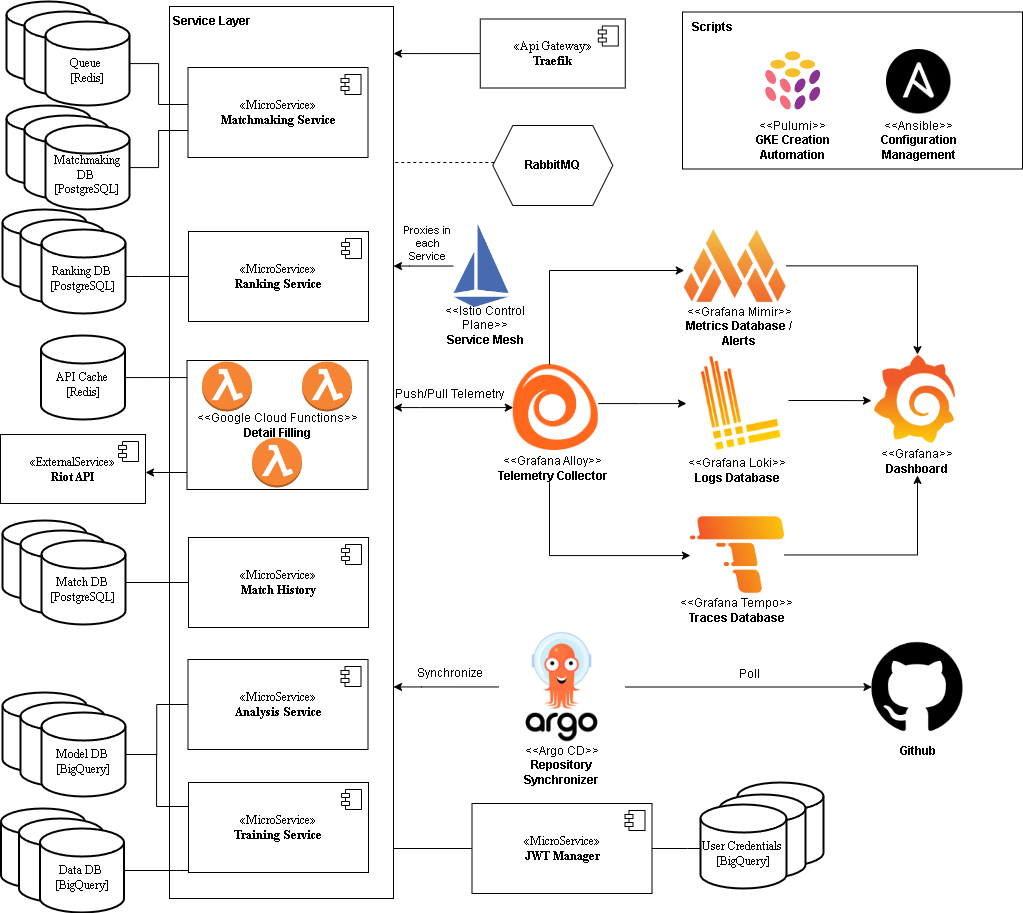
\includegraphics[width=1.0\textwidth]{../architecture/app_technical_architecture.png}
        \caption{Technical Architecture}
        \label{fig:tech-arch}
    \end{figure}

    \vspace{1cm}
    \hrule
    \vspace{1cm}

    %%%%%%%%%%%%%%%%%%%%%%%% Deployment Scripts %%%%%%%%%%%%%%%%%%%%%%%%%%%%%%%
    \section{Deployment Scripts}

    \subsection{Local Checks}
    
    \begin{lstlisting}[language=bash]
      ./scripts/format.sh
      ./scripts/test.sh
    \end{lstlisting}
    
    Python gRPC files are generated, not committed:

    \begin{lstlisting}[language=bash]
      ./scripts/python/generate-grpc.sh
    \end{lstlisting}
    
    \subsection{Deployment}
    
    Required environment:

    \begin{lstlisting}[language=bash]
        export SCRIM_PROJECT_ID="your-gcp-project"
        export SCRIM_REGION="europe-west1"
        export SCRIM_REPO_NAME="scrimfinder"
        export SCRIM_CLUSTER_NAME="scrimfinder"
        export RIOT_API_KEY="RGAPI-..."
        export SCRIM_DB_USER="scrim_admin"
        export SCRIM_DB_PASSWORD="secure_password"
    \end{lstlisting}
    
    Deploy infrastructure, images, Cloud Functions, and the Helm application:

    \begin{lstlisting}[language=bash]
        ./scripts/deploy.sh
    \end{lstlisting}
    
    Tear down the stack:

    \begin{lstlisting}[language=bash]
        ./scripts/shutdown.sh
    \end{lstlisting}

    \vspace{1cm}
    \hrule
    \vspace{1cm}

    %%%%%%%%%%%%%%%%%%%%%%%%%%%%% Tuning %%%%%%%%%%%%%%%%%%%%%%%%%%%%%%%%%%%%%%
    \section{Tuning}

    TODO - cpu/memory requests and limits, hpa, vpa, liveness and readiness checks with initialDelay/period/timeout

    \vspace{1cm}
    \hrule
    \vspace{1cm}

    %%%%%%%%%%%%%%%%%%%%%%%%%% CI/CD Pipeline %%%%%%%%%%%%%%%%%%%%%%%%%%%%%%%%%
    \section{CI/CD Pipeline}

    TODO - on push to main and work/*, on pull-request to main, test types of each and brief description of the tests, ...

    \vspace{1cm}
    \hrule
    \vspace{1cm}

    %%%%%%%%%%%%%%%% Test, Evaluation Techniques and Results %%%%%%%%%%%%%%%%%%
    \section{Test, Evaluation Techniques and Results (to target group)}

    \subsection{Documentation Feedback - Diogo Sousa}
    \begin{itemize}
        \item \bff{Style Discrepancy}: The query parameter for pagination size is documented as \texttt{pageSize} (camelCase) while the response object uses \texttt{page\_size} (snake\_case). The API Gateway correctly accepts the \texttt{pageSize} parameter and returns the corresponding schema, but this inconsistency should ideally be unified.
        \item \bff{Error Response Documentation}: While standard HTTP error codes (400, 401, 404, 500, 502) are consistently mapped across endpoints using reusable components (e.g., \texttt{BadRequestText}), they could be more descriptive. The schema indicates they return a \texttt{text/plain} string without explaining \textit{what} triggers them (e.g., what specific validation failure causes a 400, or under what conditions a 404 is thrown for a specific endpoint).
    \end{itemize}
    
    \subsection{Testing Results - Diogo Sousa}
    
    \subsubsection{Smoke Testing (Endpoint: \getapi /api/listings/search)}
    The smoke test was executed using a \bff{Python script} checking the endpoint. The test validated the HTTP 200 response, JSON validity, and the presence of all required top-level fields (\texttt{total}, \texttt{page}, \texttt{page\_size}, \texttt{listings}) and listing level attributes.
    \begin{itemize}
        \item \bff{Basic Paginated Search}: Passed. Returned 5 listings with a reported total of 50,000 records. Latency: $\approx$ 141ms.
        \item \bff{Filtered Search (Toyota Corolla)}: Passed. Returned 5 listings with a reported total of 300 records. Latency: $\approx$ 191ms.
    \end{itemize}
    No broken links or malfunctioning behaviors were detected.
    
    \subsubsection{Stress Testing (Endpoint: \getapi /api/listings)}
    The stress test was executed using \bff{Locust} against endpoint.
    \begin{itemize}
        \item \bff{Concurrency Settings}: 100 concurrent users, spawning at a rate of 20 users per second, run duration of 30 seconds.
        \item \bff{Performance observed}:
        \begin{itemize}
            \item \bff{Total Requests}: 6,899
            \item \bff{Failures}: 0 (0.00\%)
            \item \bff{Requests Per Second (RPS)}: Peaked at $\approx$ 275 req/s (average 248.81 req/s over the duration).
            \item \bff{Latency Statistics}: Average = 72ms, Median = 62ms, 95th percentile = 93ms, 99th percentile = 150ms.
        \end{itemize}
    \end{itemize}
    The endpoint proved to be highly stable under the tested load.
    
    \subsection{Documentation Feedback - Bruno Faustino}
    \begin{itemize}
        \item \bff{Some positives}:
        \begin{itemize}
            \item The API documentation was in general easy to understand due to the modularity on the groups of endpoints and the descriptive information tagged with each endpoint.
            \item The introductory paragraph gives a quick overview of all the use cases of the application and in which modules they can be found.
            \item In general, the exceptions portray in which cases the app may fail (although they could be explained in more detail according to the endpoint in some cases).
        \end{itemize}
        \item \bff{A few suggestions}:
        \begin{itemize}
            \item For the chat endpoints, a 404 code should be thrown if the chat id does not exist in the database.
            \item It would be helpful to have default values already filled-in in the body of the POST methods that serve as an example to further improve the understandability of the API (for some fields it is not trivial what the expected format is, like fuel\_type, drive\_type and end\_time).
            \item Although it is well explained that the user needs to add the Host header before calling the post/put/delete endpoints, it is never explained that the user needs to be logged in and that the resulting token needs to be added to the header: a quick mention in either the introductory paragraph or the 401 Unauthorized exception in the documentation would generate less confusion and save a few 401s.
        \end{itemize}
    \end{itemize}
    
    \subsection{Testing Results - Bruno Faustino}
    
    \subsubsection{Smoke Testing (Endpoint: \getapi /api/auctions/\{auction\_id\}/bids)}
    The smoke test was executed using \bff{pytest and requests modules of Python}.
    
    Here is the sequence of API calls as a setup before testing the actual endpoint:
    \begin{enumerate}
        \item \bff{\postapi /api/user/login} for the auth token.
        \item \bff{\postapi /api/listings} for listing\_id.
        \item \bff{\postapi /api/auctions} for auction\_id.
        \item 3x \bff{\postapi /api/auctions/\{auction\_id\}/bid}.
    \end{enumerate}
    
    After calling the endpoint: \bff{\getapi /api/auctions/\{auction\_id\}/bids}, it is expected that the command returns successfully (200) and with 3 auction bids in the created auction for the created listing.
    
    \bff{The smoke test passed!}
    
    \subsubsection{Stress Testing (Endpoint: \getapi /api/market/average\_price)}
    The stress test was executed using \bff{Locust} against the endpoint.
    \begin{itemize}
        \item \bff{Concurrency Settings}: 10000 concurrent users, spawning at a rate of 5 users per second, running until failing.
        \item \bff{Performance observed}:
        \begin{itemize}
            \item \bff{Total Requests}: 250
            \item \bff{Failures}: 4 (1.60\%)
            \item \bff{Requests Per Second (RPS)}: Very inconsistent, around 19.61 req/s.
            \item \bff{Latency Statistics}: Average = 1009ms, Median = 190ms, 95th percentile = 4000ms, 99th percentile = 6700ms.
        \end{itemize}
    \end{itemize}
    The system fails a few times at 19.61 req/s due to the unavailability of an upstream service (502).
    
    During other rounds of testing, the system could fail at less or more than that value, sometimes managing to survive without failures until around 50 req/s, so it is inconsistent, and the number of failures oscillates a lot between load tests, up to the point of reaching 99\% failures.
    
    The endpoint proved unable to sustain loads above 50 req/s, and shows signs of failing around 19.61 req/s.
    
    \subsection{Documentation Feedback - Rodrigo Neto}
    \begin{itemize}
        \item \bff{Missing Content-Type Header}: Successful JSON responses do not include the \texttt{Content-Type: application/json} header, which can break strict HTTP clients.
        \item \bff{Poor Overload Behaviour}: Under high load, the backend does not gracefully degrade (e.g., return \texttt{429} or \texttt{503}). Instead, the gateway returns \texttt{502 Bad Gateway} after extremely long timeouts (up to 47 seconds).
    \end{itemize}
    
    \subsection{Testing Results - Rodrigo Neto}
    
    \subsubsection{Smoke Testing (Endpoint: \getapi /api/market/price-comparison)}
    The smoke test was executed using \bff{Postman} checking the endpoint. The test validated HTTP 200 responses, JSON validity, pagination, grouping, and sorting behaviors.
    \begin{itemize}
        \item \bff{Happy Path}: Passed with warnings. Valid JSON, correct pagination and sorting. \texttt{Content-Type} assertion failed (header omitted).
        \item \bff{Validation}: Partial pass (3/6). Missing parameters returned 400. Invalid enum values returned \texttt{502 Bad Gateway} instead of 400.
    \end{itemize}
    Some malfunctioning behaviors were detected during validation tests.
    
    \subsubsection{Stress Testing (Endpoint: \getapi /api/listings/stats/by-location)}
    The stress test was executed using \bff{Locust} against the endpoint.
    \begin{itemize}
        \item \bff{Concurrency Settings}: Step-load ramping from 10 to 200 concurrent users.
        \item \bff{Performance observed}:
        \begin{itemize}
            \item \bff{Total Requests}: 3,524
            \item \bff{Failures}: 123 (3.49\%)
            \item \bff{Requests Per Second (RPS)}: Peaked at $\approx$ 50 req/s.
            \item \bff{Latency Statistics}: Average = 7,280ms, Median = 460ms, 95th percentile = 34,000ms, 99th percentile = 38,000ms.
        \end{itemize}
    \end{itemize}
    The endpoint proved unable to sustain loads above $\approx$ 50 RPS, leaving the upstream backend in an unhealthy state.

    \vspace{1cm}
    \hrule
    \vspace{1cm}

    %%%%%%%%%%%% Corrections Implemented after Feedback from Testing %%%%%%%%%%
    \section{Corrections Implemented after Feedback from Testing}

    TODO

    \vspace{1cm}
    \hrule
    \vspace{1cm}

    %%%%%%%%%%%%%%%%%%%%%%%%%% Cost Analysis %%%%%%%%%%%%%%%%%%%%%%%%%%%%%%%%%%
    \section{Cost Analysis}

    TODO

    \vspace{1cm}
    \hrule
    \vspace{1cm}

    %%%%%%%%%%%%%%%%%%%%%%%%%%% Conclusions %%%%%%%%%%%%%%%%%%%%%%%%%%%%%%%%%%%
    \section{Conclusions}

    TODO

    \vspace{1cm}
    \hrule
    \vspace{1cm}

\end{document}
